\chapter{拡散性の評価}

\section{評価基準}
1章でも述べた通り、ホール空間は吸音面が1階客席面に偏在する非完全拡散音場である。
ここで、座席面遠方音場は大きな吸音力を持つ座席面から離れることにより、音場がより拡散した状態になるという推測のもと、拡散性の観点から評価を行う(\figref{far_improve})。
\\ さて、関連した用語として従来より残響理論の仮定として用いられる「完全拡散音場」がある。これは、次の2条件を満たす音場のことである。
\\(i)音響エネルギが室内全体に均一に分布していること。
\\(i\hspace{-.05em}i)どの点においても音の進行方向があらゆる方向に一様であること。
\\ 物理的な拡散性を言及するにあたり上記2条件を拡散性評価の軸とする。すなわち、(i)で音響エネルギ分布の一様性を、(ii)で反射音方向分布の一様性を評価する。各評価項目を\figref{kakusan}に示す。
\\ 以上を基に、本研究では物理的評価に立脚した音場の拡散性評価を行う。
\vspace{0.8cm}
\begin{figure}[htbp]
    \centering
    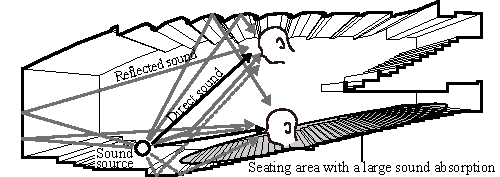
\includegraphics[keepaspectratio,scale=1.7]{01_att/concert_ear.pdf}
    \caption{\hspace{1mm}The difference of directional uiformity}
    \label{fig:far_improve}
\end{figure}

\section{評価手法}
オーディトリウムで得られた測定値を観測高さごとに定量化するため、統計的手法を用いる。
\subsection{平均値}
その室の全観測点から算出した平均値は単一の値で音響特性を言い表す便利な値である。
しかしながら、残響時間を除く多くの音響物理量(明瞭性や音量感など)の平均値は観測位置により大きく異なる値から算出される可能性があるため$^{\text{\cite{barron2005using}}}$、用いる際にはその室における全体の分布をみる必要がある。また、これは音響性能が全く異なる2つのホールが同じ平均値を取りうることを意味する。Barronは好意的な主観的印象を得るホールと聴衆にあまり受け入れられないホールの2つの例を示し、両ホールにおける主観的印象の平均値はほんのわずかな違いであったと述べている$^{\text{\cite{barron2002value}}}$。すなわち、主観的印象が全く異なるにも関わらず、ホールの平均値が非常に近い値をとる場合がある。
\subsection{標準偏差}

音響エネルギ分布の一様性を定量的に評価するため、標準偏差を用いた評価を行う。

\subsection{一元配置分散分析}
観測高さごとの音響物理量の違いをみるため、一元配置分散分析を用いる。これは、要因が異なる複数の標本の母平均が等しい(複数の標本から求められた平均値が、同じ母平均を持つ母集団から抽出された)という仮説を検定することにより、要因の違いにより複数の標本の母平均に違いがあるか(要因の違いに意味があるか)を検討するものである$^{\text{\cite{kanno}{\cite{池田1}{\cite{池田2}{\cite{池田3}}}}}}$。
\\ 観測点(x,y,$H_z$)における室内音響物理指標・音響物理量が観測高さ$H$により受ける影響を調べるため一元分散分析(対応あり)を用いて分析を行う。また、分析によって有意差が確認できた指標についてはHolm法による多重比較を行う。

\subsection{室内音響物理指標の弁別限}
水準間に有意な差があったとき、その差は人間が知覚できるほどの変化量であるかどうかをJND ( just noticeable difference : 感覚上ちょうど感知できる物理刺激の最小変化量 ) を用いて判断する。
ISO3382-1$^{\text{\cite{iso3382}}}$に整理されている室内音響物理指標の弁別限(JND)を\tabref{jnd}に示す。
\begin{table}[htbp]
\centering
\caption{\hspace{1mm}JND of each acoustic parameters}
\label{tab:jnd}
\begin{tabular}{lccc}
\Hline
\multicolumn{1}{c}{Subjective listener aspect} & Acoustic quantity & \begin{tabular}[c]{@{}c@{}}Single number\\ freq. ave.$^*${[}Hz{]}\end{tabular} & \begin{tabular}[c]{@{}c@{}}Just noticeable difference\\ (JND)\end{tabular} \\ \hline
Subjective level of sound & $G${[}dB{]} & 500 to 1000 & 1[dB] \\
Perceived reverberance & $EDT${[}s{]} & 500 to 1000 & Rel.5[\%] \\
Perceived clarity of sound & $C_{80}${[}dB{]} & 500 to 1000 & 1[dB] \\
" & $D_{50}${[}\%{]} & 500 to 1000 & 5{[}\%{]} \\
Apparent source width (ASW) & $LF${[}\%{]} & 500 to 1000 & 5{[}\%{]} \\
\Hline
\multicolumn{4}{l}{$^{*}$ : The single number frequency averaging denotes the arithmetical average for the octave bands.}
\end{tabular}
\end{table}

\pagebreak
\subsection{室内音圧レベル分布に関する理論値}
従来の室内音響理論においては、拡散音の音圧レベルは距離によらず一定になる。
しかし、コンサートホールの実測調査では、これに当てはまらない結果を示すものがあった。
そこでBarronは拡散音が距離によって減衰するという修正理論$^{\text{\cite{barron1988energy}}}$を提案している。
\\ Barron's revised theoryではインパルス応答を直接音($d$)、初期反射音領域($e_r$ : t \textless 80 ms)、後期反射音領域($l$ : t \textgreater 80 ms)と時間軸上で分けて扱っている。ここで、$r$は音源-観測点間距離[m]、$T$は残響時間[s]、$V$は室容積[m$^3$]を表す。
\begin{table}[htbp]
    \begin{equation}
        \label{eq:d}
        d=\frac{100}{r^2}
    \end{equation}
    \begin{equation}
        e_r=\frac{31200T}{V}e^{\frac{-0.04r}{T}}(1-e^{\frac{-1.11}{T}})
    \end{equation}
    \begin{equation}
        l=\frac{31200T}{V}e^{\frac{-0.04r}{T}}e^{\frac{-1.11}{T}}
    \end{equation}
\end{table}
\\ $d$、$e_r$、$l$を用いて室内音響物理指標$G$や$C_{80}$、及び$G_{early}$,$G_{late}$の理論値が算出可能となる。以後、音場の評価を行う際はBarron's revised theoryによる理論値との比較検討を行う。
\begin{table}[htbp]
    \begin{equation}
        G=10\log_{10}(d+e_r+l)\hspace{2mm}\dB
    \end{equation}
    \begin{equation}
        G_{early}=10\log_{10}(d+e)\hspace{2mm}\dB
    \end{equation}
    \begin{equation}
        G_{late}=10\log_{10}(l)\hspace{2mm}\dB
    \end{equation}
    \begin{equation}
        C_{80}=10\log_{10}(\frac{d+e_r}{l})\hspace{2mm}\dB
    \end{equation}

%        \begin{equation}
%        G_{early}=10\log_{10}(d+e_r)\hspace{2mm}\dB
%    \begin{equation}
%        VG_{early}=LG_{early}=GG_{early}=10\log_{10}\frac{d+e_r}{3}\hspace{2mm}\dB
%   \end{equation}
\end{table}